\pagestyle{empty}
\cleardoublepage
\pagestyle{fancy}

\chapter{Resultados}\label{cap6}

\section{Resultados dos experimentos}\label{cap6:intro}

Foram usadas três diferentes máquinas para testar o algoritmo, apresentado na tabela \ref{table: machines}. Maquina A tem uma CPU i7 a20, com 4 cores com velocidade de clock de 2,67 GHz, 8192 MB de cache, 8 GB de RAM and 2 nVidia GTX 295, cada GTX 295 tem 280 cores por GPU, clock da memória de 999 MHz e tamanho da banda de memória de 223,8 GB/segundos com 2 GPUs em cada. Maquina B  tem um i7 4930K CPU, com 6 cores, clock de 3,4 GHz, memoria cache de 12288 KB, 32 GB de RAM e 2 nVidia GTX 680, GTX 680 tem 1546 cores, 6 Gbps clock de memória e tamanho da banda de memória de 192,2 MHz. Máquina C tem um CPU i7 3939K, com 6 cores, velocidade de clock de 3,2 GHz, memória cache de 12288KB, 32 GB de RAM e 1 nVidia GTX Titan, GTX Titan tem 2688 cores, velocidade da memória de 6 Gbps e tamanho da banda de memória de 223,8 GB/segundo. Foram considerados os cenários com apenas a máquina A, com a máquina A, e com a três máquinas (A, B e C). Os computadores estão conectados por uma rede Gigabit Ethernet. Foi usado o sistema operacional Ubuntu 12.04 e CUDA 5.5.


\begin{table}[!t]
\centering
\tiny
\caption{Configuração das máquinas}

\begin{tabular}{|c|c|c|c|c|}
\hline
\multicolumn{1}{|l|}{Máquina} & Modelo CPU  & Número de GPUs & \multicolumn{1}{l|}{Memória da GPU } & Modelo de GPU \\ \hline
A                             & Intel i7 a20   & 4 x GTX200b         & 896MB                          & GTX 295   \\ \hline
B                             & Intel i7 4930K  & 2 x GK104           & 2GB                            & GTX 680   \\ \hline
C                             & Intel i7 3930K & 2 x GK110     & 6GB                            & GTX Titan \\ \hline
\end{tabular}
\label{table: machines}
\end{table}


Para usar todos os n multiprocessadores da GPU, é necessário criar ao menos n blocos. Mais que isso, cada multiprocessador simultaneamente executa grupos (chamados de warps) de m threads de um único bloco. e muitos warps estão presentes em cada GPU para o uso eficiente dos processadores.

Em todos os testes, usa-se todos os multiprocessadores das GPUs lançando kernels com $k$ blocos com 1024 threads por bloco, onde $k$ é o numero de processadores na GPU. Para as GPUs usadas, $k$ é 14, 8 e 30 na GTX Titan, GTX 680 e GTX 295 respectivamente. Para as CPUs, foram usados todos os cores das CPUs, lançando uma tarefa pro core.

 \section{Multiplicação de Matrizes}

O algoritmo foi testatdo para a multiplicação de matrizes usando uma, duas e três máquinas e quatro diferentes algoritmos de escalonamento: (1) algoritmo proposto, (2) estático, (3) HDSS, e (4) StarPU (guloso).

\begin{figure}[htb]
	\begin{center}
	\centering
			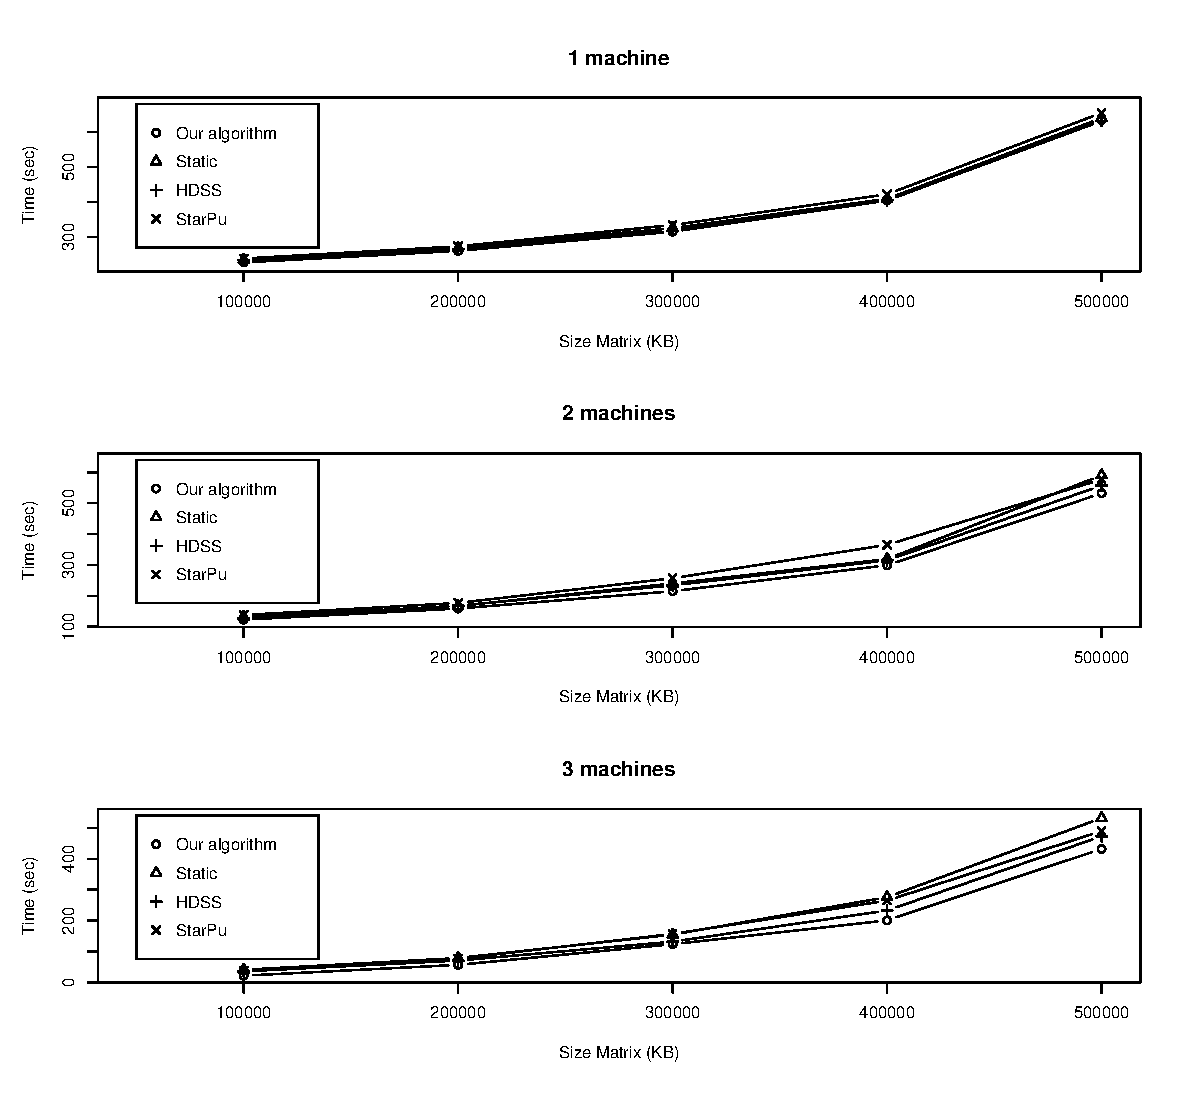
\includegraphics[scale=0.459]{EmbaixoNovo.eps}
	\caption{Diferença de execução com diferentes tamanhos de matrizes, para a multiplicação de matrizes}
	\label{fig:todosJuntos}
	\end{center}
\end{figure}

A figure \ref{fig:todosJuntos} apresenta os resultados para matrizes com tamanhos 10.000 x 10.000 a 50.000 x 50.000. Em todos os cenários, o algoritmo de escalonamento proposto obteve melhores resultados, com o HDSS em segundo. O estático e o StarPU foram claramente inferiores.

Com uma máquina a diferença foi pequena porque há poucos tipos de dispositivos para o escalonador selecionar. Com duas máquinas nosso algoritmo começa a ter melhor desempenho, especialemente para casos de matrizes grandes, que é explicado pelo fato de que o tempo de execução da maultiplicação de matrizes aumenta rapidamente como aumenta-se o tamanho da matriz. Com três máquinas obteve-se o ambiente mais heterogêneo e o ganho de desempenho usando o algoritmo proposto é o maior. Como nos outros cenários, aumentando-se o tamanho da matriz também aumenta-se o ganho de desempenho como o algoritmo proposto. Para matrizes 10.000 x 10.000, o algoritmo proposto gastou 20 segundos enquanto o HDSS gastou 36, que resulta em 22,2\% mais rápido. E para matrizes 50.000 x 50.000, o algoritmo proposto gastou 433 segundos enquanto o HDSS 473, que resulta em 8,49\% mais rápido, o resumos está na tabela \ref{able: comparativo}

\begin{table}[h]
\centering
\tiny
\caption{Comparativo: HDSS x Algoritmo Proposto}

\begin{tabular}{c|c|c|c|c|c|c|}
\cline{2-7}
\multicolumn{1}{l|}{}                 & \multicolumn{3}{c|}{Tamanho Matriz 10,000 x 10,000 KB}                     & \multicolumn{3}{c|}{tamanho Matriz 50,000 x 50,000 }                                       \\ \hline
\multicolumn{1}{|l|}{Num. Máquinas} & HDSS   & Algoritmo Proposto& \multicolumn{1}{l|}{Differ. (\%)} & \multicolumn{1}{l|}{HDSS} & Algoritmo Proposto& \multicolumn{1}{l|}{Differ. (\%)} \\ \hline
\multicolumn{1}{|c|}{1 Machine}       & 233.42 & 227.01        & 2.75                                 & 632.13                    & 635.32        & -0.50                                \\ \hline
\multicolumn{1}{|c|}{2 Machines}      & 129.43 & 123.62        & 4.49                                 & 557.92                    & 532.11        & 4.63                                 \\ \hline
\multicolumn{1}{|c|}{3 Machines}      & 36.85  & 22.43         & 39.13                                & 473.64                    & 433.41        &            8.49                          \\ \hline
\end{tabular}
\label{table: comparativo}
\end{table}

Os resultados obtidos mostram que em ambientes mais heterogêneos o uso do algoritmo proposto apresenta mais vantagem. Esta vantagem é devido melhor distribuição dos dados ao longo da execução. A figura \ref{fig:diferencaThreads} mostra a diferença de tempo entre a primeira e a última thread, no cenário com três máquinas.

\begin{figure}[htb]
	\begin{center}
	\centering
			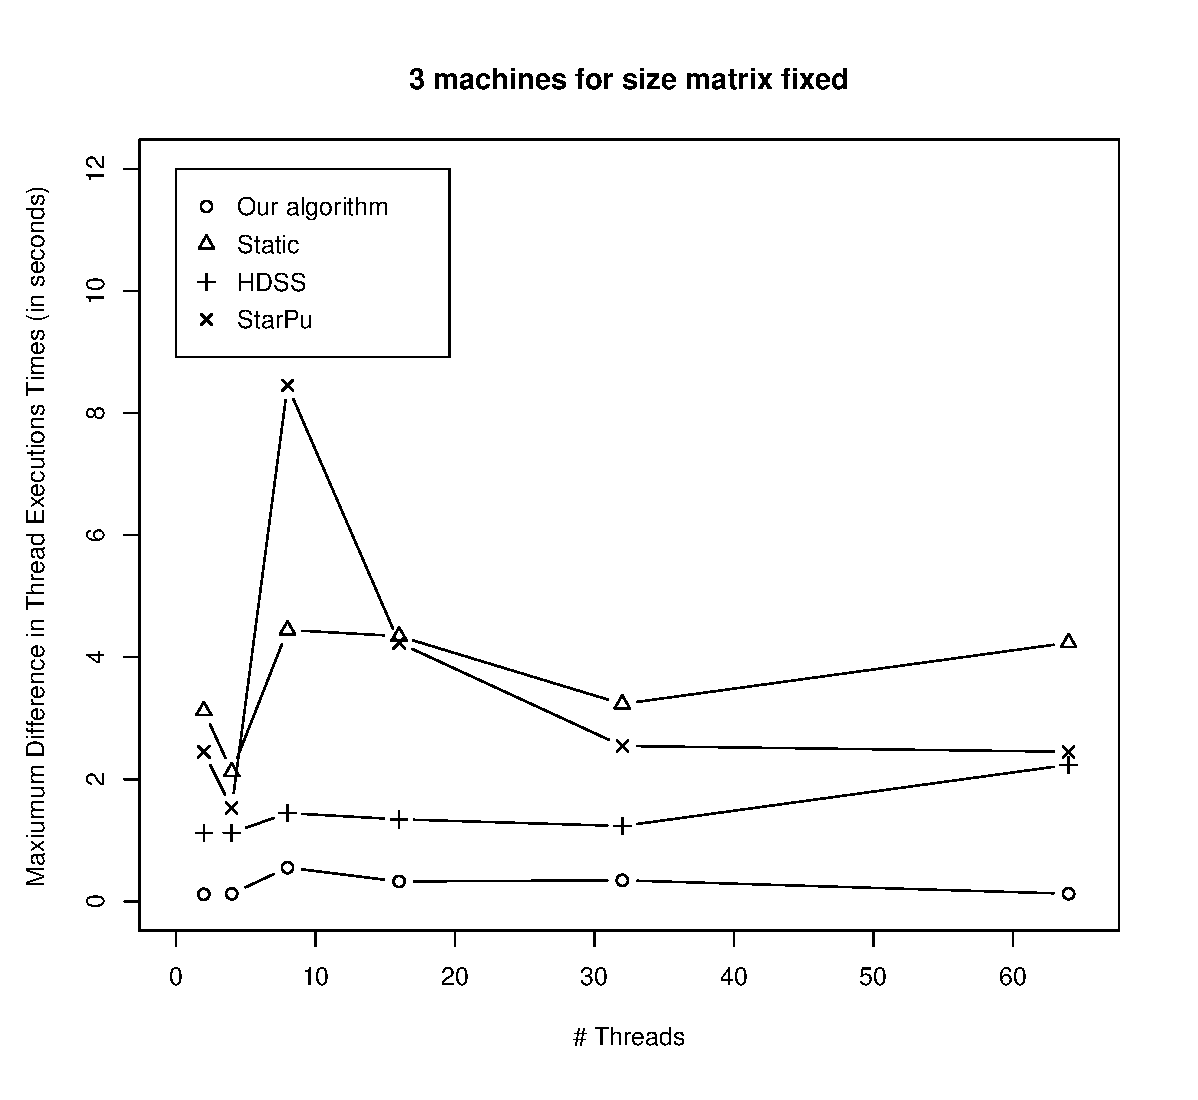
\includegraphics[scale=0.4]{MaximaDiferenca.eps}
	\caption{Diferença de tempo entre Threads}
	\label{fig:diferencaThreads}
	\end{center}
\end{figure}

O algoritmo guloso do StarPU teve um bom desempenho, considerando que ele não tem diretamente a informação sobre a velocidade de processamento dos dispositivos. Mas ele usa estas informações indiretamente, desde que dispositivos mais rápidos que terminam suas tarefas mais cedo e, consequentemente, recebem mais tarefas. O algoritmo estático teve o pior desempenho, porque deixa a thread ociosa por muito tempo ver figura \ref{fig:diferencaThreads}. Há grandes diferenças entre final de threads. 


HDSS utiliza o início da execução para estimar o melhor tamanho de bloco e usa essa distribuição até o fim da execução. Além disso, grandes blocos são usados no início da execução, 
causando um atraso maior devido ao desbalanço quando usa diferentes tipos de dispositivos, 
como GPUs e CPUs. Por fim, HDSS utiliza uma aproximação bruta para a capacidade do dispositivo.

O algoritmo proposto tem  bastante precisão na estimativa,  a quantidade de dados que devem ser 
fornecida para cada unidade de processamento, a solução de um problema de optimização com o 
restrição de que todas as unidades devem terminar a execução das tarefas ao mesmo 
tempo. Quando a diferença entre terminar a execução de threads para certos 
partição de dados excede um certo limite, o algoritmo reequilibra os dados 
distribuição.

\section{Blackscholes}

\begin{figure}[htb]
	\begin{center}
	\centering
			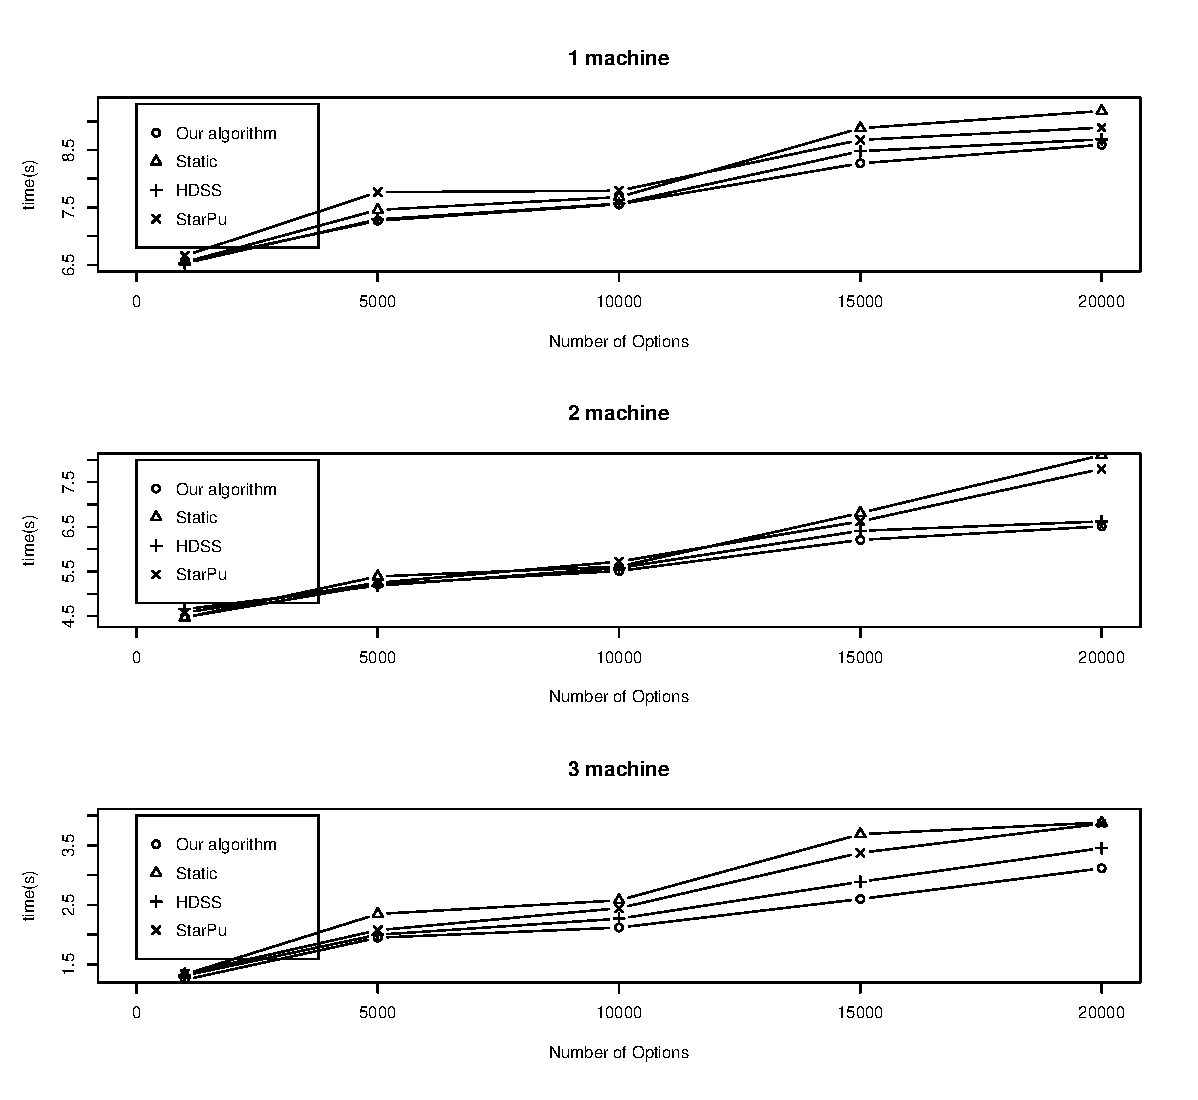
\includegraphics[scale=0.459]{MaquinaBlack.eps}
	\caption{Diferença no tempo de execução para diferentes números de opção}
	\label{fig:black}
	\end{center}
\end{figure}

Foram realizados testes de tempo de execução para a aplicação chamada blackscholes usando diferentes configuraçõs de máquinas. A figura~\ref{fig:black} apresenta os tempo de execução, onde variou-se o número de opõs em cada execução e obteve-se o tempo de execução. Similarmente aos experimentos de multiplicação de matrizes, o melhor desempenho foi alcançado nos problemas maiores, com maior números de opções e em ambientes mais heterogêneos. Os resultados podem ser explicados com os mesmos argumentos. Blackscholes tem complexidade linear com o número de opções, mostrando que o algoritmo proposto é também útil para esta classe de problemas. A tabela  \ref{table: black} mostra os valores extremos com 1000 e 20000 opções, o melhor resultado foi com três máquinas, e com o maior número de opções.

\begin{table}{h}
\centering
\tiny
\caption{Comparativo: HDSS x Algoritmo Proposto}

\begin{tabular}{c|c|c|c|c|c|c|}
\cline{2-7}
\multicolumn{1}{l|}{}                 & \multicolumn{3}{c|}{1000 Opções}                              & \multicolumn{3}{c|}{20000 Opções}                                                  \\ \hline
\multicolumn{1}{|l|}{Num. Máquinas} & HDSS (s) & Algoritmo (s) & \multicolumn{1}{l|}{Diff. (\%)} & \multicolumn{1}{l|}{HDSS (s)} & Algoritimo (s) & \multicolumn{1}{l|}{Diff. (\%)} \\ \hline
\multicolumn{1}{|c|}{1 }       & 6.52     & 6.55              & -0.45                           & 8.68                          & 8.59              & 1,03                            \\ \hline
\multicolumn{1}{|c|}{2 }      & 4.65     & 4.47              & 3.87                            & 6.62                          & 6.51              & 1.66                            \\ \hline
\multicolumn{1}{|c|}{3 }      & 1.31     & 1.24              & 5.34                            & 3.45                          & 3.11              &               9.81                  \\ \hline
\end{tabular}
\label{table: black}
\end{table}

Também, considerou-se que a aplicação termina em menos que 4 segundos, para o cenário com 3 máquinas, é possível notar que o \emph{overhead} imposto pelo solucionador do sistema de equações para determinar a melhor distribuição é pequeno e o ganho obtido ultrapassa o custo dos cálculos. Para as aplicações testadas, em poucas iterações, foi possível obter a solução do sistema de equações, o que resultou em poucos milissegundos, na ordem de 10 ms.

\begin{figure}[htb]
	\begin{center}
	\centering
			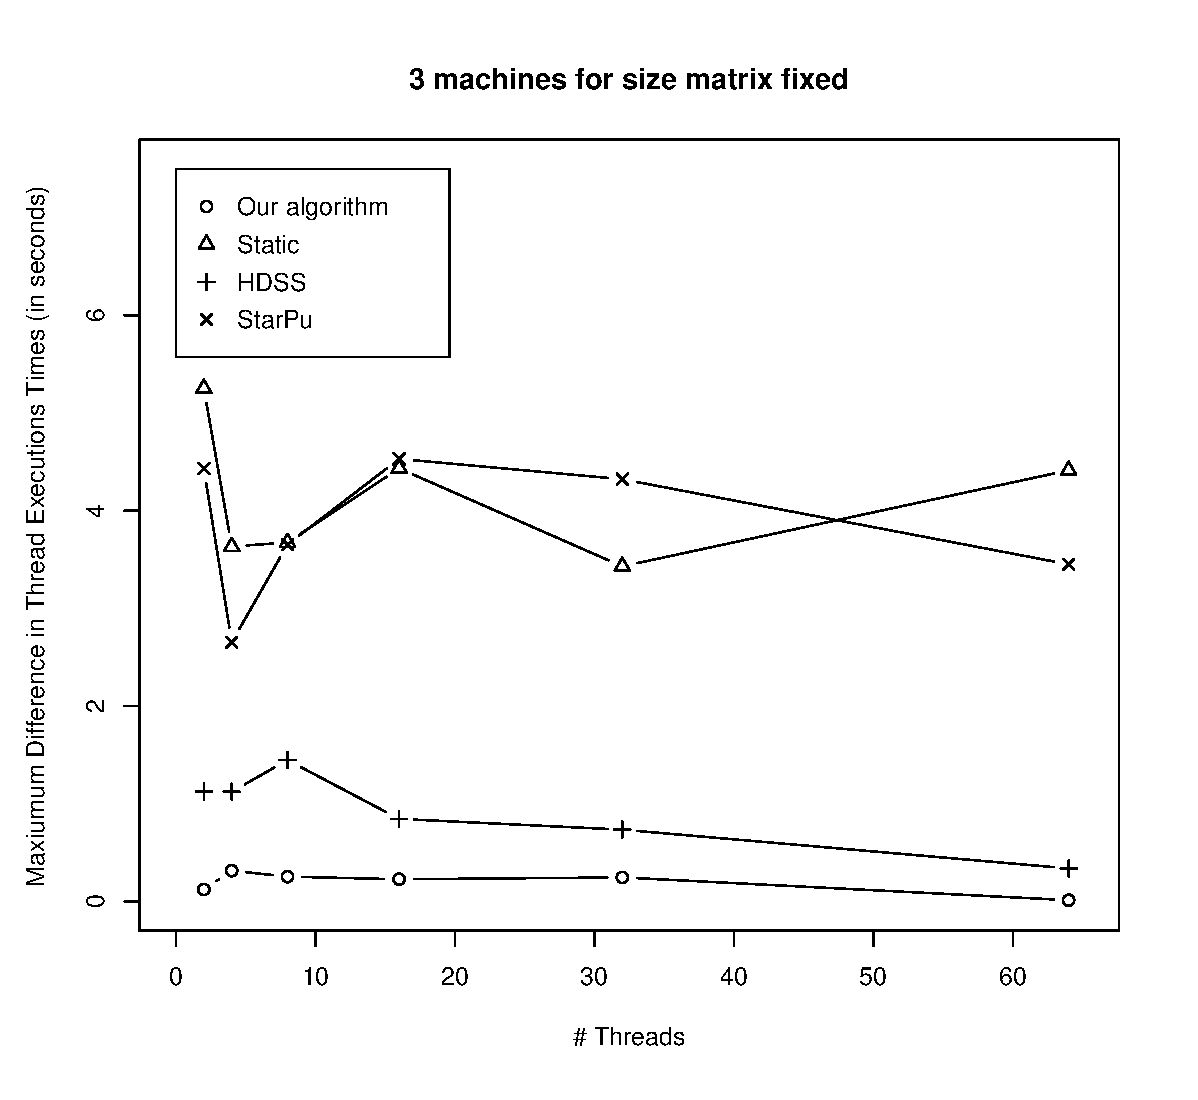
\includegraphics[scale=0.4]{MaximaDiferencaBlack.eps}
	\caption{Diferença de tempo entre a primeira e a última thread a terminarem o trabalho}
	\label{fig:diferencaThreadsBlack}
	\end{center}
\end{figure}

A figura~\ref{fig:diferencaThreadsBlack} confirma o resultado de que a diferença entre a primeira a terminar  e a última, no cenário com três máquinas é sempre menor para o algoritmo proposto.


\section{Conclusões}\label{cap6:conclusao}

Foi proposto um algoritmo de escalonamento de tarefas para problemas de decomposição de domínio que executam em \emph{clusters} de CPUs e GPUs hetererogêneas. O algoritmo proposto supera outros algoritmos similares devido a estimativa online da curva de desempenho para cada  processador e a seleção da melhor distribuição para os dispositivos. foi apresentado para duas aplicações que o algoritmo proposto fornece maiores ganhos para problemas grandes e em ambientes mais heterogêneos.

Embora usou-se clusters dedicados, pode-se também considerar o uso em nuvem públicas, onde o usuário pode requisitar um numero de recursos alocados me máquinas virtuais de máquinas compartilhadas. Neste caso, a qualidade do serviço pode alterar durante a execução, e a adição de um limiar permite ajustar a distribuição de dados. Pode-se também considerar o ceneario com a adição de tolerância a falhas, onde máquinas podem ser tornar indisponíveis durante a execução. Neste cenário, uma simples redistribuição dos dados entre os dispositivos restantes permitiria que a aplicação ser readapte a este cenário.




